\section{Correlation Analysis}
\begin{frame}{The Experiment}
\begin{itemize}
    \item Correlation between the encryption time of PRESENT algorithm and the number of set bits in the key.
    \item Generate random messages of 64 bit and corresponding to each message generate random keys with count of set bits varying from 1 to 79.
\end{itemize}
\end{frame}
\begin{frame}{The Experiment Cont..}
\begin{center}
        \begin{figure}[h!]
            \minipage{0.5\textwidth}
              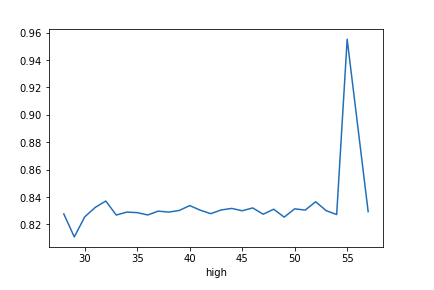
\includegraphics[width=0.8\linewidth]{CA1.PNG}
            \endminipage\hfill
            \minipage{0.5\textwidth}
              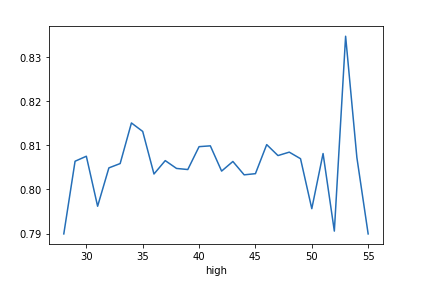
\includegraphics[width=0.8\linewidth]{CA2.PNG}
            \endminipage
        \end{figure}
    \end{center}
    \begin{center}
        \begin{figure}[h!]
            \minipage{0.5\textwidth}
              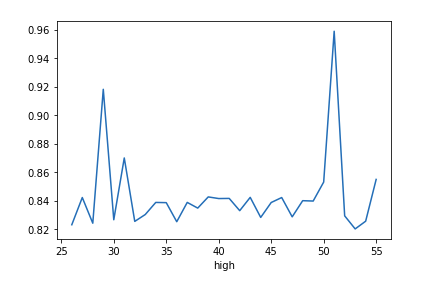
\includegraphics[width=0.8\linewidth]{CA3.PNG}
            \endminipage\hfill
            \minipage{0.5\textwidth}
              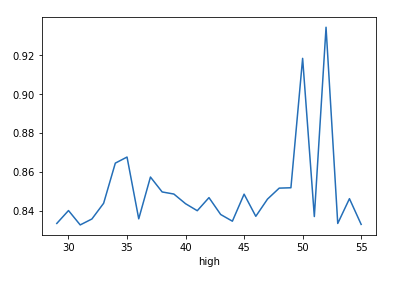
\includegraphics[width=0.8\linewidth]{CA4.PNG}
            \endminipage
        \end{figure}
    \end{center}
\end{frame}
\begin{frame}{The Experiment Cont..}
\begin{center}
        \begin{figure}[h!]
            \minipage{0.5\textwidth}
              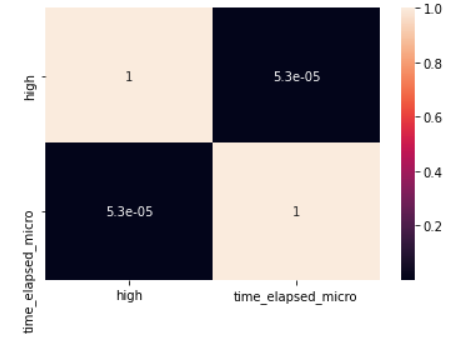
\includegraphics[width=0.8\linewidth]{heatmap.PNG}
            \endminipage\hfill
            \minipage{0.5\textwidth}
              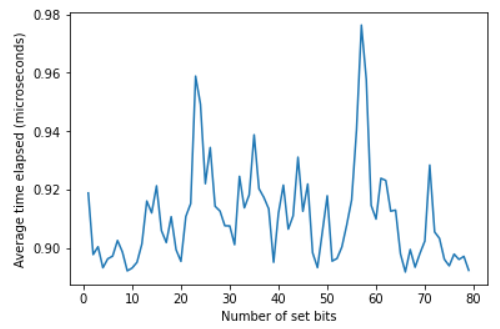
\includegraphics[width=0.8\linewidth]{lineplot.PNG}
            \endminipage
        \end{figure}
    \end{center}
\begin{itemize}
    \item Near to zero correlation exists.
    \item No or very weak linear relationship between the variables.
\end{itemize}
\end{frame}